%Poster do trabalho de conclusao de curso 

\documentclass[final]{beamer}
\mode<presentation>{\usetheme{azul}}
\usepackage{graphicx}
\usepackage{epstopdf}
\usepackage{subfigure}

\usepackage[brazil]{babel}
\usepackage[utf8]{inputenc}
\usepackage{ragged2e} 

\usepackage[T1]{fontenc}
\usepackage[justification=centering]{caption}


\usepackage{amsmath,amsthm, amssymb, latexsym}
\usepackage[orientation=portrait,size=a2,scale=1.4]{beamerposter}
\usepackage[ruled]{algorithm2e}

\usepackage{snapshot} % will write a .dep file with all dependencies, allows for easy bundling

\DeclareMathSizes{17.42}{15}{14}{10}  % Math text size

%%%%%%%%%%%%%%%%%%%%%%%%%%%%%%%%
%%  MACROS %%%%%%%%%%%%%%%%%%%%%
\usepackage{xspace}
\newcommand{\pixel}{\emph{pixel}\xspace}
\newcommand{\pixels}{\emph{pixels}\xspace}
\newcommand{\voxel}{\emph{voxel}\xspace}
\newcommand{\voxels}{\emph{voxels}\xspace}


\listfiles
%%%%%%%%%%%%%%%%%%%%%%%%%%%%%%%%%%%%%%%%%%%%%%%%%%%%%%%%%%%%%%%%%%%%%%%%%%%%%%%%%%%%%%
\title{\huge Etherclan - Rede distribuída descentralizada para localização de outros usuários}

\author{Henrique Gemignani Passos Lima <henrique@gemignani.org>, Orientador: Prof. Dr. Daniel Macêdo Batista}
\institute[Universidade de São Paulo] % (optional, but mostly needed)
{
  Instituto de Matemática e Estatística, Universidade de São Paulo - Trabalho
  de Conclusão de Curso
}

\date[Novembro 2013]{Novembro, 2013}
%%%%%%%%%%%%%%%%%%%%%%%%%%%%%%%%%%%%%%%%%%%%%%%%%%%%%%%%%%%%%%%%%%%%%%%%%%%%%%%%%%%%%%
\newlength{\columnheight}
\setlength{\columnheight}{65cm}
%%%%%%%%%%%%%%%%%%%%%%%%%%%%%%%%%%%%%%%%%%%%%%%%%%%%%%%%%%%%%%%%%%%%%%%%%%%%%%%%%%%%%%
\begin{document}
\begin{frame}
  \begin{columns}
    % ---------------------------------------------------------%
    % Set up a column 
    \begin{column}{.5\textwidth}
      \begin{beamercolorbox}[center,wd=\textwidth]{postercolumn}
        \begin{minipage}[T]{.95\textwidth} % tweaks the width, makes a new \textwidth
          \parbox[t][\columnheight]{\textwidth}{ % must be some better way to set the the height, width and textwidth simultaneously
            % Since all columns are the same length, it is all nice and tidy.  You have to get the height empirically
            % ---------------------------------------------------------%
            % fill each column with content            
            
            \vspace*{0.8cm}
            
            \begin{block}{Introdução}
            \justifying
                Desenvolvedores de jogos eletrônicos livres que desejam implementar alguma
                funcionalidade multijogador sofrem com um problema: manter servidores, ou pelo
                menos uma lista desses. Jogos comerciais mais antigos para PC adotavam a
                estratégia de permitir que o jogador se conectasse a um endereço IP qualquer.
                Também era popular o jogo ter um lista de servidores oficial, que podia ser
                acessada de dentro do jogo. Já jogos comerciais recentes sempre possuem um
                servidor oficial principal do qual todas funcionalidades multijogador dependem.
                
                \vspace*{0.15cm}
                
                No caso de um jogo livre, o desenvolvedor tem duas opções: manter ele mesmo um
                servidor principal ou deixar esse trabalho para a comunidade. O primeiro implica
                num custo de manutenção para o desenvolvedor, enquanto o segundo aumenta a
                barreira de entrada para novos jogadores, dado que o jogador precisa ativamente
                procurar tal lista.
                
                \vspace*{0.15cm}

                \textbf{Neste trabalho, propomos uma rede distribuída descentralizada na qual
                todos os jogadores e servidores participam como uma solução alternativa.}
                
                \vspace*{0.2cm}
            \end{block}
            
            \vspace*{0.2cm}

            \begin{block}{Objetivos}
              \justifying
              \begin{itemize}
                \item Desenvolver uma rede peer-to-peer com o propósito de permitir que usuários do jogo consigam encontrar outros jogadores,
                sem a necessidade de um servidor central. 
                
                \vspace*{0.4cm}
                
                \item Implementar pelo menos 1 prova de conceito.
              \end{itemize}
              \vspace*{0.2cm} 
            \end{block}
            
            \vspace*{0.2cm}
            
            \begin{block}{Rede peer-to-peer}
                \center 
                \begin{figure}[h]
                  \fbox{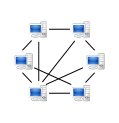
\includegraphics[width=0.45\textwidth]{p2p-network.png}}
                  \fbox{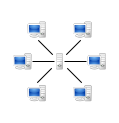
\includegraphics[width=0.45\textwidth]{server-based-network.png}}
                  \caption{Comparação de rede Peer-to-peer (Esquerda) com Cliente-Servidor (Direita). 
                    Fonte: Baseado em figura de Wikimedia Commons}
                \end{figure}
                                
                \vspace*{0.2cm}
            \end{block}
            
            \vspace*{0.2cm}

            \begin{block}{Protocolo de Rede}
            \justifying
                Quando mensagens são trocadas através de uma rede de computadores seguindo um sistema de regras digitais,
                tal sistema é chamado de um protocolo de rede. Sistemas de comunicação usam formatos bem-definidos para
                trocar mensagens. 
                
                \vspace*{0.4cm} 
                
                \begin{figure}[h]
                  \fbox{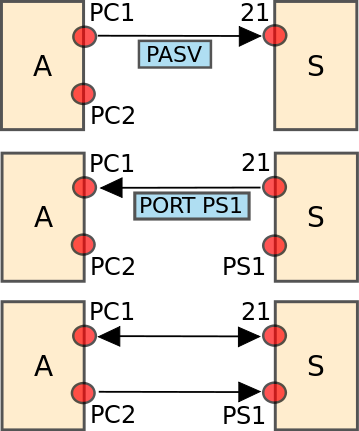
\includegraphics[width=0.4\textwidth]{passive_ftp_connection.png}}
                  \caption{Exemplo de fluxo de mensagens no protocolo FTP.
                    Fonte: Wikimedia Commons}
                \end{figure}
                
                \vspace*{0.2cm} 
                
                Cada mensagem tem um significado exato intencionado a provocar uma resposta particular
                do receptor. Portanto, o protocolo define a sintaxe, semânticas, e sincronização da comunicação. Protocolos
                de comunicação devem ser acordados por todas as partes envolvidas.
                               
                \vspace*{0.2cm} 
            \end{block}
          }
        \end{minipage}
      \end{beamercolorbox}
    \end{column}
    % ---------------------------------------------------------%
    % end the column

    % ---------------------------------------------------------%
    % Set up a column 
    \begin{column}{.5\textwidth}
      \begin{beamercolorbox}[center,wd=\textwidth]{postercolumn}
        \begin{minipage}[T]{.95\textwidth} % tweaks the width, makes a new \textwidth
          \parbox[t][\columnheight]{\textwidth}{ % must be some better way to set the the height, width and textwidth simultaneously
            % Since all columns are the same length, it is all nice and tidy.  You have to get the height empirically
            % ---------------------------------------------------------%
            % fill each column with content
            
            \vspace*{0.8cm}
            
            \begin{block}{Etherclan}
                A rede Etherclan é uma rede Peer-to-Peer com o objetivo de permitir que algum cliente
                encontre outros clientes
                pertinentes. Ela tem as seguintes propriedades:
                
                \begin{itemize}
                  \item Não depende de um servidor centralizado.
                  \item Pode ser utilizada por mais de um jogo simultaneamente.
                  \item Capaz de buscar por membros de um jogo específico.
                \end{itemize}
                
                \vspace*{0.5cm}
                Para que os nós consigam conversar entre si, foi necessário definir um protocolo. 
                Nele, foram existem as seguintes mensagems:
                \begin{itemize}
                  \item ANNOUNCE\_SELF -- Anuncia a própria existência para o receptor.
                  \item REQUEST\_NODE\_LIST -- Requisita do receptor uma lista de nós da rede.
                  \item KEEP\_ALIVE -- Avisa que vai enviar mais mensagens nessa mesma conexão.
                  \item SERVICE -- Comando para ser tratado usando alguma extensão definida por terceiros.
                \end{itemize}
                
                \vspace*{0.2cm}
                
                E a seguinte resposta possível:
                \begin{itemize}
                  \item NODE\_INFO -- Informações sobre um nó da rede.
                \end{itemize}
                
                \vspace*{0.2cm} 
            \end{block}

            \vspace*{0.2cm} 
            
            \begin{block}{Resultados: Chat}
              \justifying 
                Como prova de conceito, foi implementado um programa de conversação que utiliza a rede para enviar e receber
                mensagens de outros nós. As mensagens são enviadas para todos e sem nome, com o único identificador sendo o IP
                de origem.
                
                \begin{figure}[htp]
                  \centering
                   \fbox{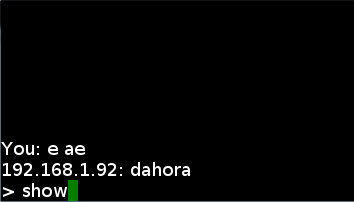
\includegraphics[width=0.7\textwidth]{chat.png}}
                  \caption{Chat em funcionamento}
                \end{figure}
                \begin{figure}[htp]
                  \centering
                   \fbox{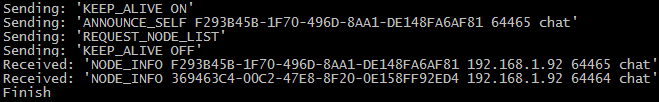
\includegraphics[width=0.95\textwidth]{chat-log.png}}
                  \caption{Log das mensagens enviadas e recebidas durante a descoberta de nós}
                \end{figure}
                
                \vspace*{0.4cm}
                
                Resultados obtidos com esse exemplo incluem:
                \begin{itemize}
                  \item Funciona! É possível conseguir encontrar a rede inteira através de alguns nós.
                  \item Problemas com NAT. Sem adotar pelo menos UPnP, torna-se impraticável o uso para encontrar nós atravéz da Internet.
                  \item É necessário ter boas escolhas em quando iniciar novas buscas por nós, assim como por quanto tempo executar a busca.
                  \item Nós não avisam quando eles ficam offline, então algum critério para decidir se um nó deixou de existir é importante.
                \end{itemize}
                
                \vspace*{0.2cm}
            \end{block}
            
            \vspace*{0.2cm} 
            \begin{block}{Trabalhos Futuros}
                Durante o desenvolvimento do protocolo e principalmente da prova de conceito, vários pontos se mostraram fundamentais e que serão estudados no futuro.
                
                \begin{itemize}
                  \item Política de quantos outros nós buscar.
                  \item Política de quando que um nó é considerado morto e deve ser ignorado.
                  \item Diminuir a complexidade de para quais nós devo perguntar para algo melhor que O(n).
                  \item Desenvolvimento de uma biblioteca em C++ para facilitar a integração com outros projetos.
                \end{itemize}
                
                \vspace*{0.2cm} 
            \end{block}
            
            %\vspace*{0.2cm} 
            %
            %\begin{block}{Referências}
            %  \small
            %    \begin{itemize}
            %        \item Rüdiger Schollmeier, A Definition of Peer-to-Peer Networking for the Classification of Peer-to-Peer Architectures and Applications, Proceedings of the First International Conference on Peer-to-Peer Computing, IEEE (2002).
            %    \end{itemize}
            %    \vspace*{0.2cm} 
            %\end{block}
            \vfill
          }
        \end{minipage}
      \end{beamercolorbox}
    \end{column}
    % ---------------------------------------------------------%
    % end the column


  \end{columns}
\end{frame}

\end{document}


%%%%%%%%%%%%%%%%%%%%%%%%%%%%%%%%%%%%%%%%%%%%%%%%%%%%%%%%%%%%%%%%%%%%%%%%%%%%%%%%%%%%%%%%%%%%%%%%%%%%
%%% Local Variables: 
%%% mode: latex
%%% TeX-PDF-mode: t
%%% End:
